\section{Signalfilterung}
In diesem Abschnitt soll die Signalfilterung genauer betrachtet werden. Dafür wird wieder der Ausgang des Generators mit dem Eingang des Analog-Digital-Wandlers verbunden. Parallel dazu wird der Ausgang des Generators mit dem Oszilloskop überwacht.

\subsection{Verschiedene Tiefpassfilterkurven}
\label{sec:VerTi}
Zuerst sollen die Filterkurven verschiedener Tiefpässe dargestellt werden. Hierzu wird am Generator ein Sinussignal ($f=100$\,Hz) mit einer Rauschbandbreite von 20\,MHz eingestellt.\\

%Für einen groben Überblick und um Unterschiede besser erkennen zu können werden alle Filterkurven in einem gemeinsamen Diagramm dargestellt (Abbildung \ref{fig:43aAll}). \\

\begin{center}
    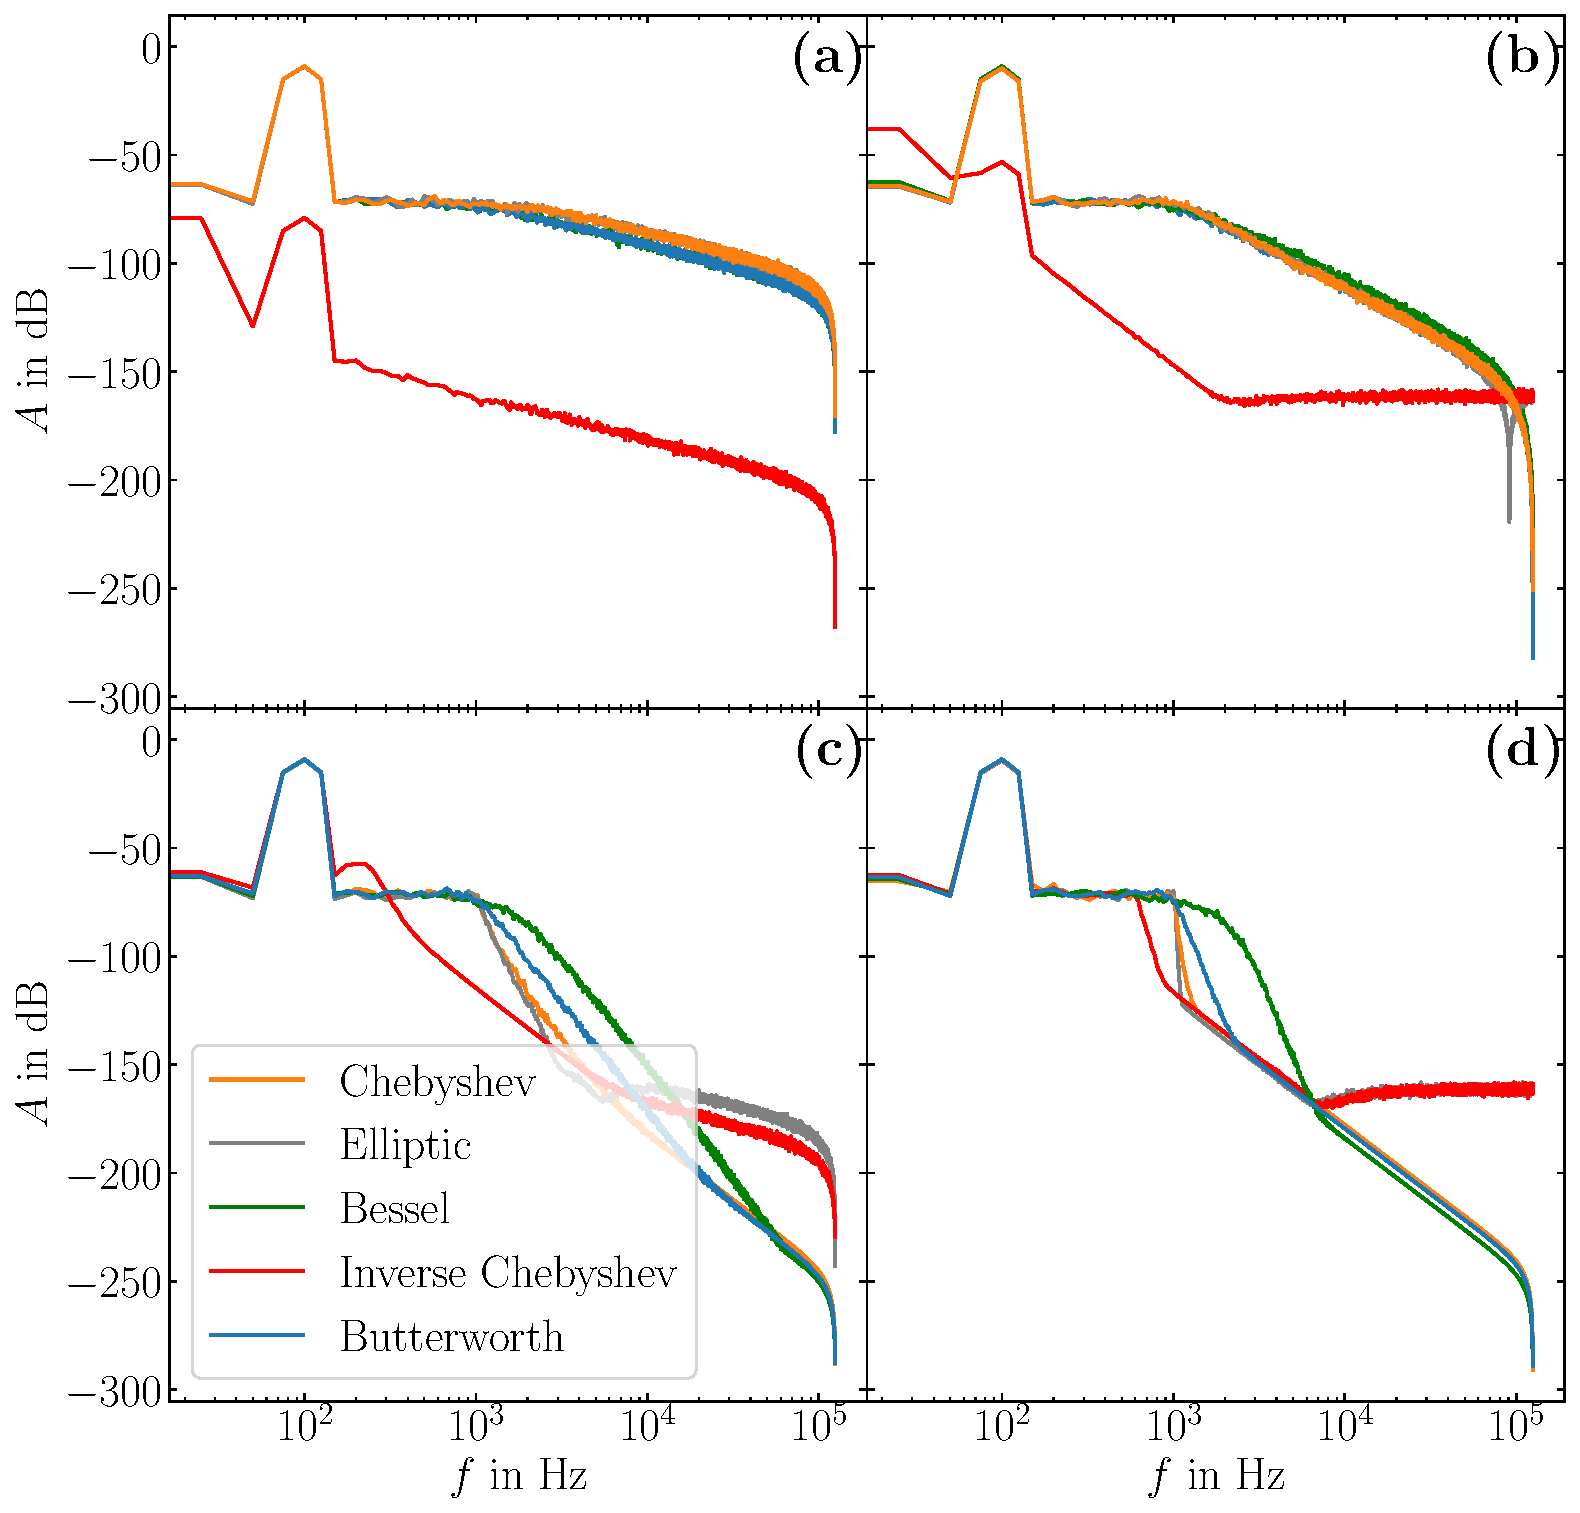
\includegraphics[width = 0.9\textwidth]{Paul/43aAllOrAll.pdf}
    \captionof{figure}{Fourierspektrum verschiedene Tiefpassfilter mit (a) Ordnung 1, (b) Ordnung 2, (c) Ordnung 5 und (d) Ordnung 10}
    \label{fig:43aAll}
\end{center}

In Abbildung \ref{fig:43aAll} fällt auf, dass sich Elliptic- und Chebyshevfilter fast deckungsgleich überlagern. Auch Butterworth- und Besselfilter sind fast deckungsgleich mit den oben genannten lediglich für Frequenzen zwischen ca. $1\cdot 10^3$\,Hz und $1\cdot 10^5$\,Hz divergieren sie geringfügig. Am stärksten weicht der inverse Chebyshevfilter von den anderen ab. Der Verlauf ist sehr ähnlich, nahezu parallel, jedoch ist sie Kurve nach unten verschoben. Für höhere Ordnungen fallen die Kurven nach dem Knick immer steiler ab und die Kurven nähern sich im Durchgansbereich an, wärend sie für hohe Frequenzen stärker von einander abweichen. Genaueres im Bezug auf die Ordnung wird in Abschnitt \ref{chap:Einfl-d-Ord} beschrieben.\\

%\newpage
Außerdem soll  für jede Filterkurve der 3\,dB-Punkt und die Steigung, für große Frequenzen bestimmt werden.
Dies wurde mithilfe des Diagramms ermittelt.

\begin{table}[h]
    \centering
    \begin{tabular}[h]{l|c|c|c}
        Filter      & \makecell{3dB-Punkt\\in Hz} & \makecell{Steigung\\ in dB/Oktave} & \makecell{Steigung\\ in dB/Dekade} \\ \hline
        Butterworth &    $1994\pm50$   &        $4\pm2$        &      $16\pm4$         \\
        Chebyshev   &    $1975\pm50$   &        $3\pm3$        &      $13\pm4$         \\
        inverser Chebyshev &$1499\pm50$&        $4\pm2$        &      $19\pm3$         \\
        Elliptic    &     $1499\pm50$  &        $3\pm4$        &      $15\pm6$         \\
        Bessel      &     $1801\pm50$  &        $4\pm2$        &      $17\pm4$         \\
    \end{tabular}
    \caption{Werte des 3dB-Punktes und der Steigung für verschiedene Filter}
    \label{tab:Stei}
\end{table}
Aus dem Vorbereitungsgespräch, mit dem Betreuer, ist bekannt, dass für einen Filter erster Ordnung 6\,dB/Oktave (oder 20\,dB/Dekade) erwartet werden. Trotz einiger Abweichungen stimmen die Größenordnungen, der Werte aus Tabelle \ref{tab:Stei} gut überein. Die großen Fehler sind der graphischen Werteermittlung geschuldet, für eine grobe Beurteilung, ob die vorliegende Messung Sinn ergib, war dies jedoch ausreichend.




\newpage
\subsection{Filterwirkung auf Rechtecksignal}
In diesem Abschnitt soll die Wirkung verschiedener Filter auf ein Rechtecksignal\\ ($f=100$\,Hz) untersucht werden.\\
Hierfür wurde der Butterworthfilter und der inverse Chebyshevfilter ausgewählt, da dieser in Abschnitt \ref{sec:VerTi} die größte Abweichung von den anderen zeigte.

\begin{figure}[h]
    \centering
    \begin{subfigure}{0.9\textwidth}
        \centering
        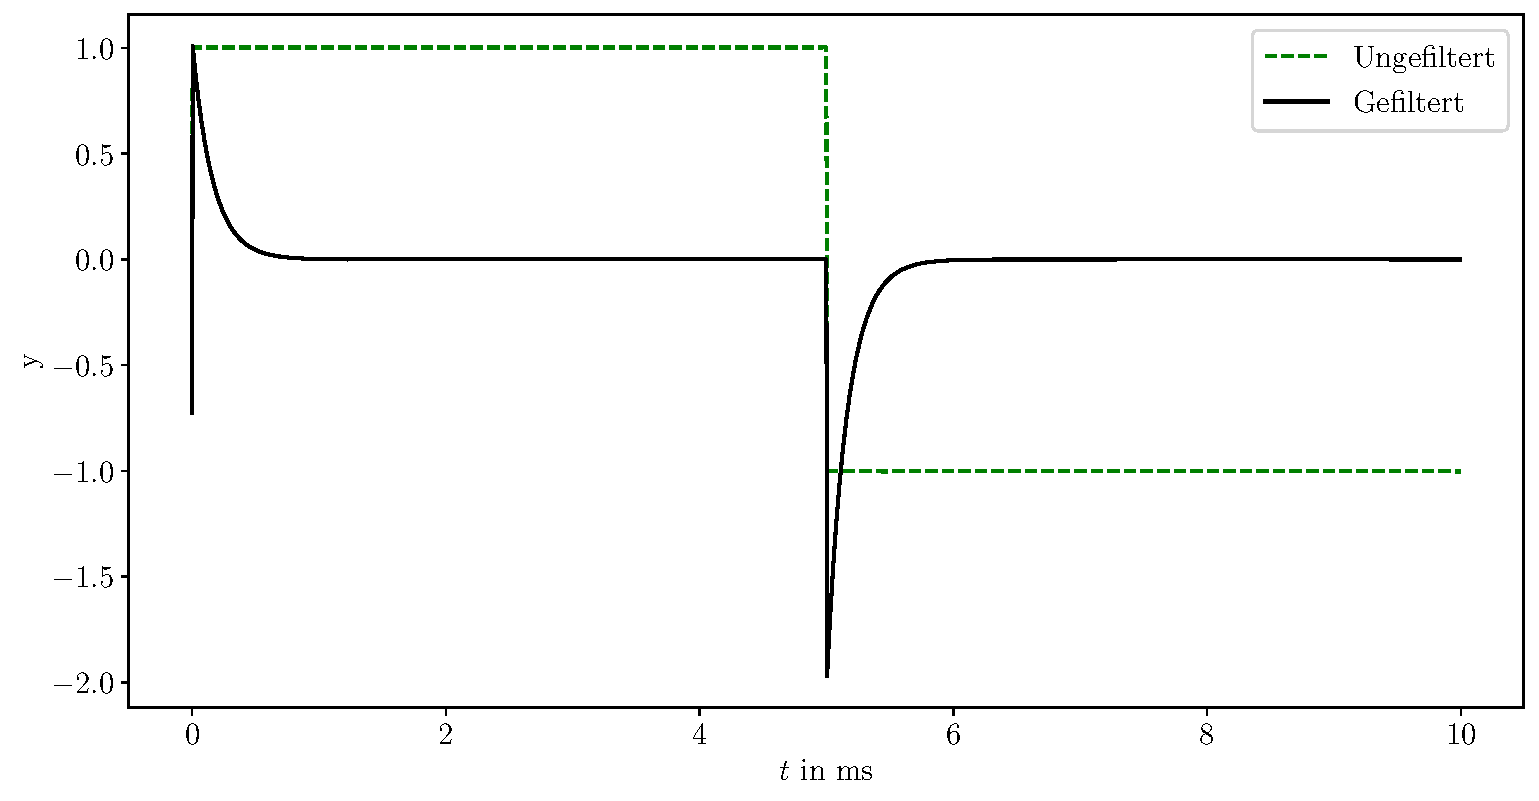
\includegraphics[width=\textwidth]{Paul/43bBuHi1S.pdf}
        \caption{Signal}
    \end{subfigure}
    \\
    \begin{subfigure}{0.9\textwidth}
        \centering
        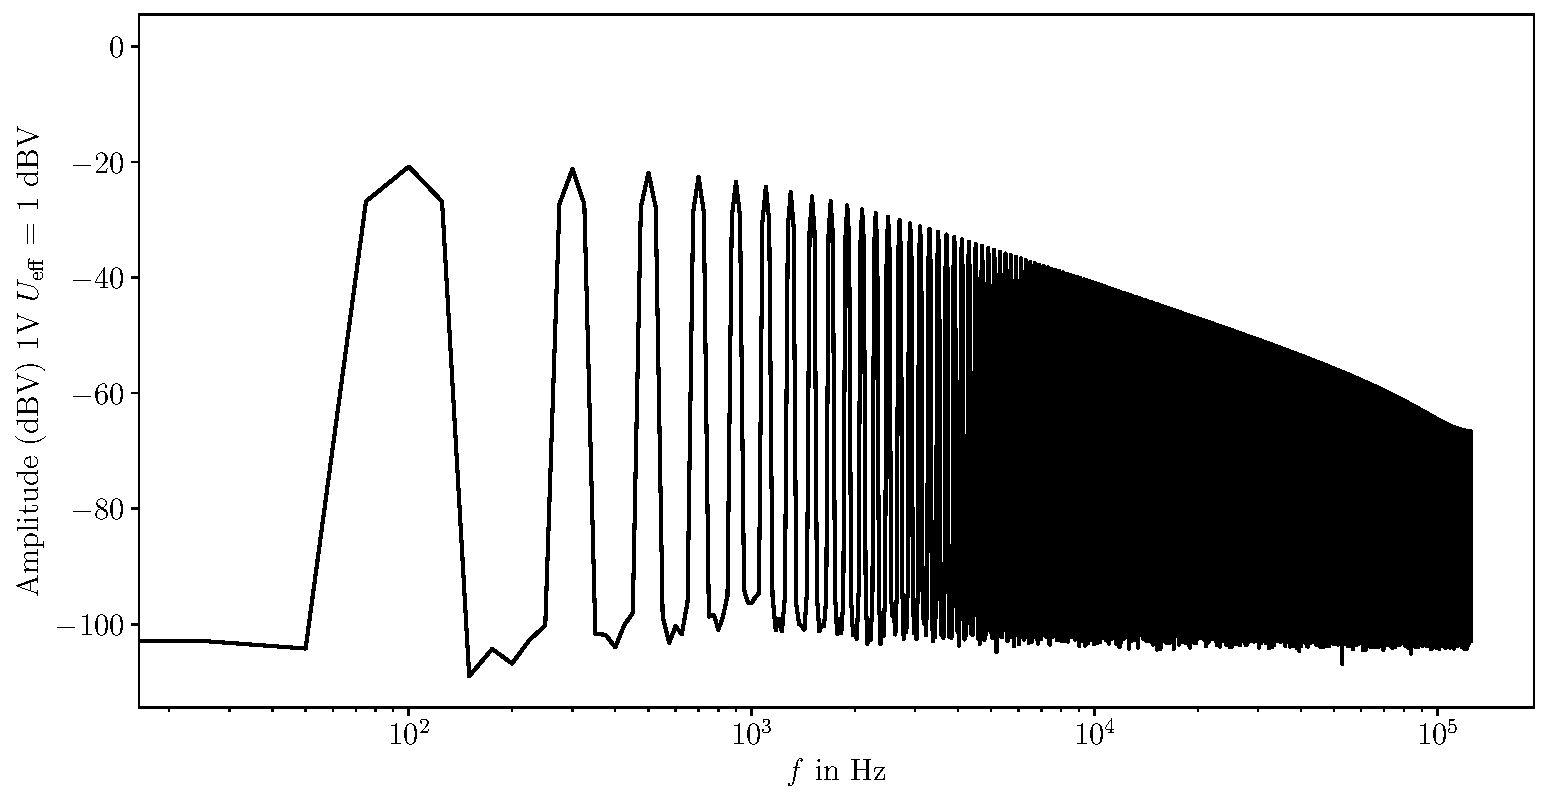
\includegraphics[width=\textwidth]{Paul/43bBuHi1F.pdf}
        \caption{Fourierspektrum}
    \end{subfigure}
    \caption{Butterworthfilter als Hochpass}
    \label{fig:43bBuHi1}
\end{figure}

Aus Abbildung \ref{fig:43bBuHi1} geht klar die differenzierende Eigenschaft des Hochpasses hervor. Außerdem knickt das Fourierspektrum für große Frequenzen ab.\\

\begin{figure}[h]
    \centering
    \begin{subfigure}{0.9\textwidth}
        \centering
        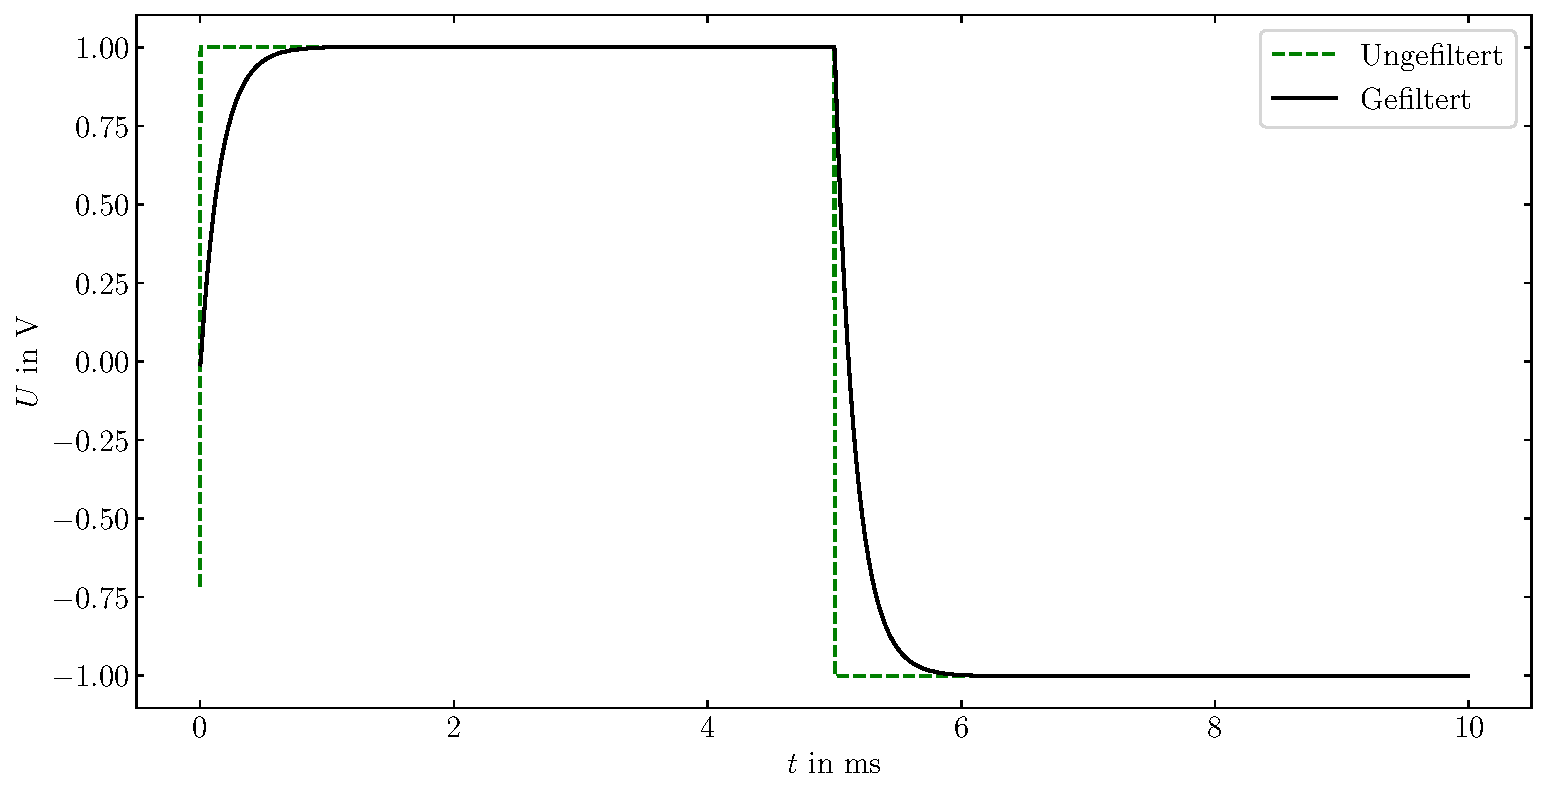
\includegraphics[width=\textwidth]{Paul/43bBuLo1S.pdf}
        \caption{Signal}
    \end{subfigure}
    \\
    \begin{subfigure}{0.9\textwidth}
        \centering
        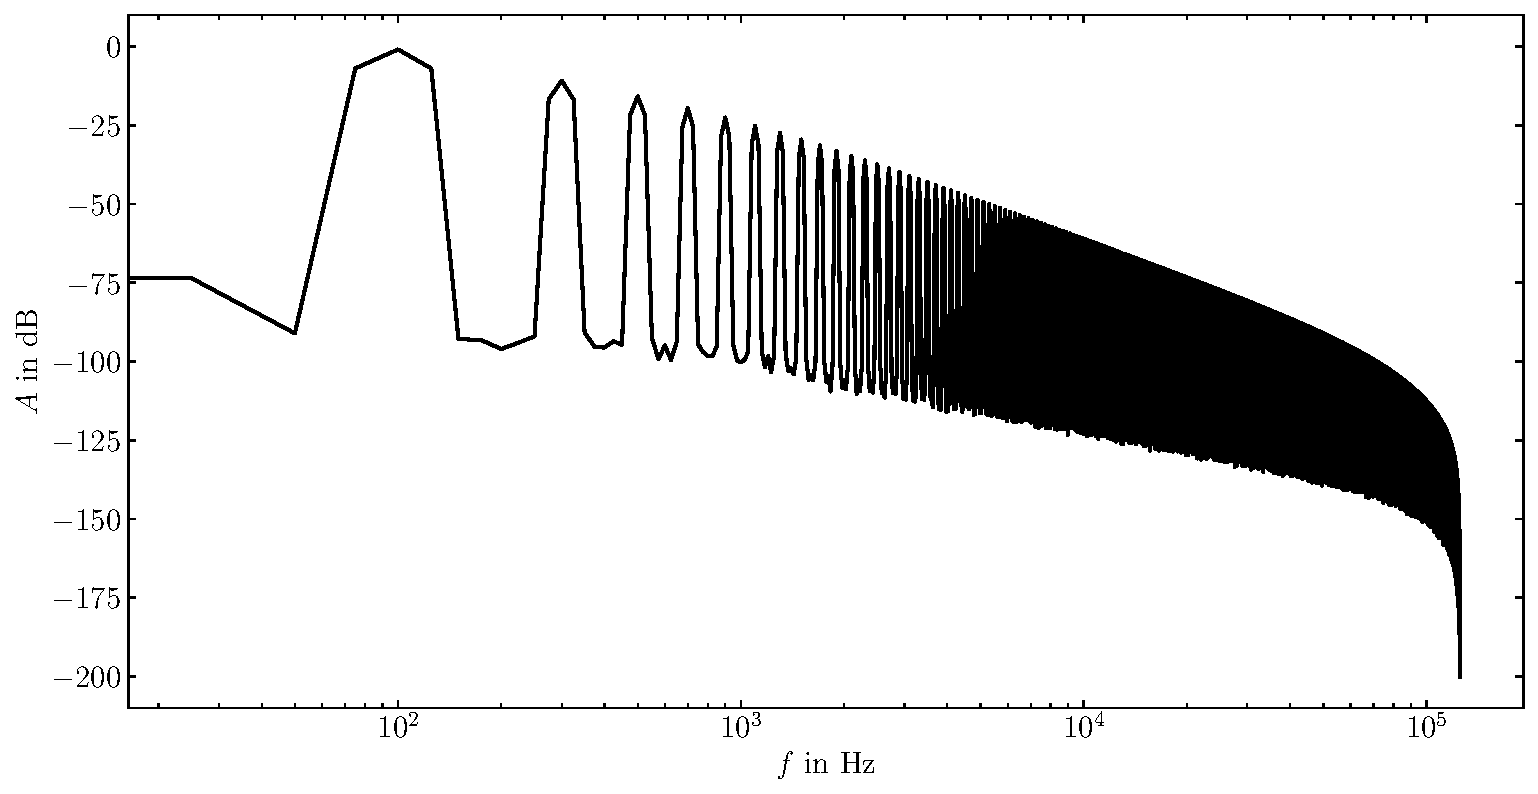
\includegraphics[width=\textwidth]{Paul/43bBuLo1F.pdf}
        \caption{Fourierspektrum}
    \end{subfigure}
    \caption{Butterworthfilter als Tiefpass}
    \label{fig:43BuLo1}
\end{figure}

Im Gegensatz zum Hochpass wirkt der Butterworthfilter Tiefpass als Integriere und das Fourierspektrum knickt für große Frequenzen ab, dies ist in Abbildung \ref{fig:43BuLo1} zu erkennen.


\newpage
Der inverse Chebyshevfilter zeigt vor allem im Signal ein ganz anderes Bild.\\
In Abbildung \ref{fig:43bInChHi1} ist beim Signal in der ersten Millisekunde eine gewisse Welligkeit zu erkennen. Im Bezug auf das Fourierspektrum fällt auf das dieser Filter, im Vergleich zum Butterworthhochpass, für größere Frequenzen schneller durchlässiger wird.
\begin{figure}[h]
    \centering
    \begin{subfigure}{0.9\textwidth}
        \centering
        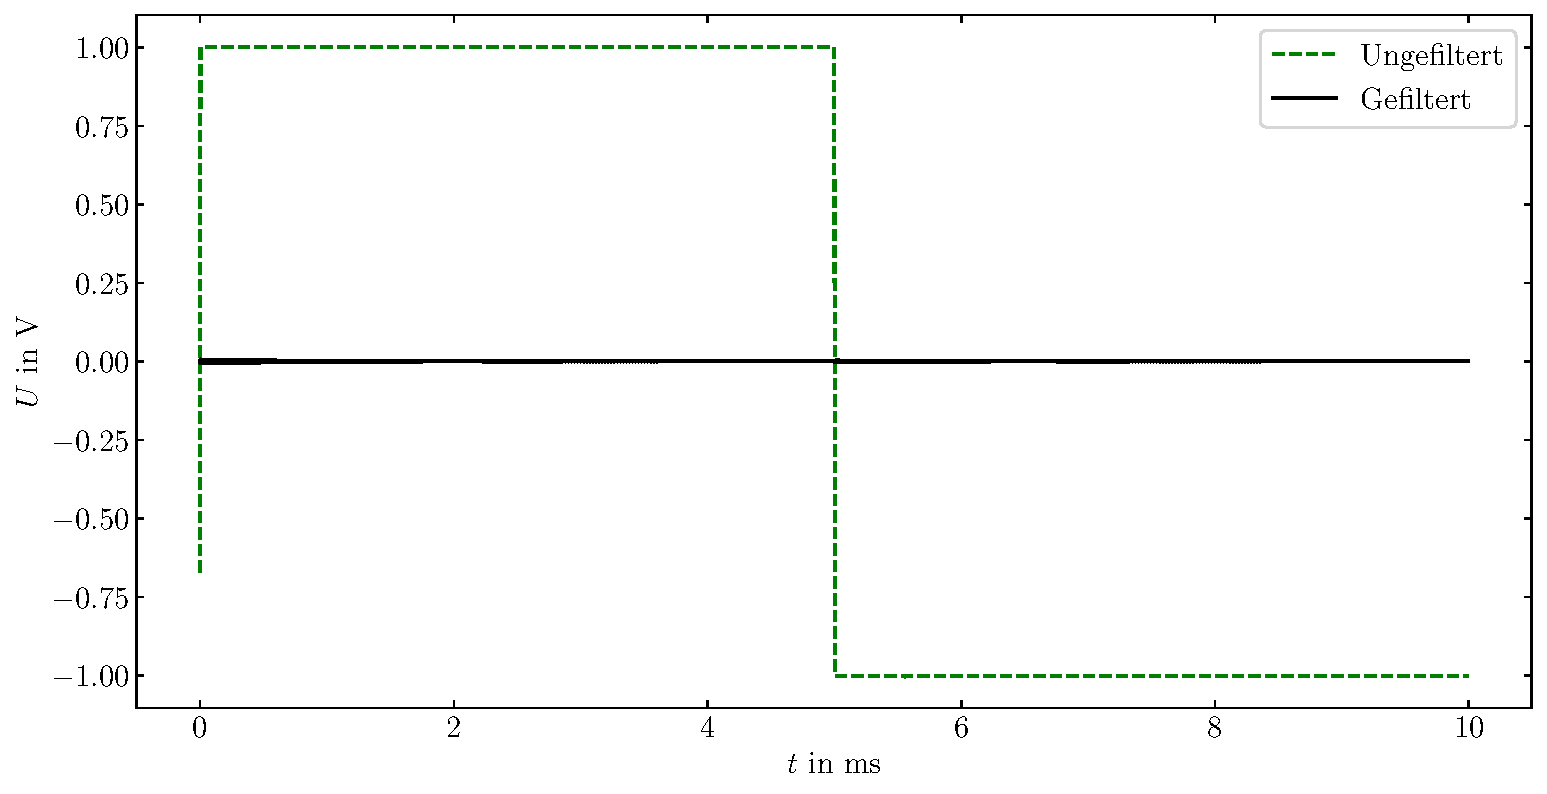
\includegraphics[width=\textwidth]{Paul/43bInChHi1S.pdf}
        \caption{Signal}
    \end{subfigure}
    \\
    \begin{subfigure}{0.9\textwidth}
        \centering
        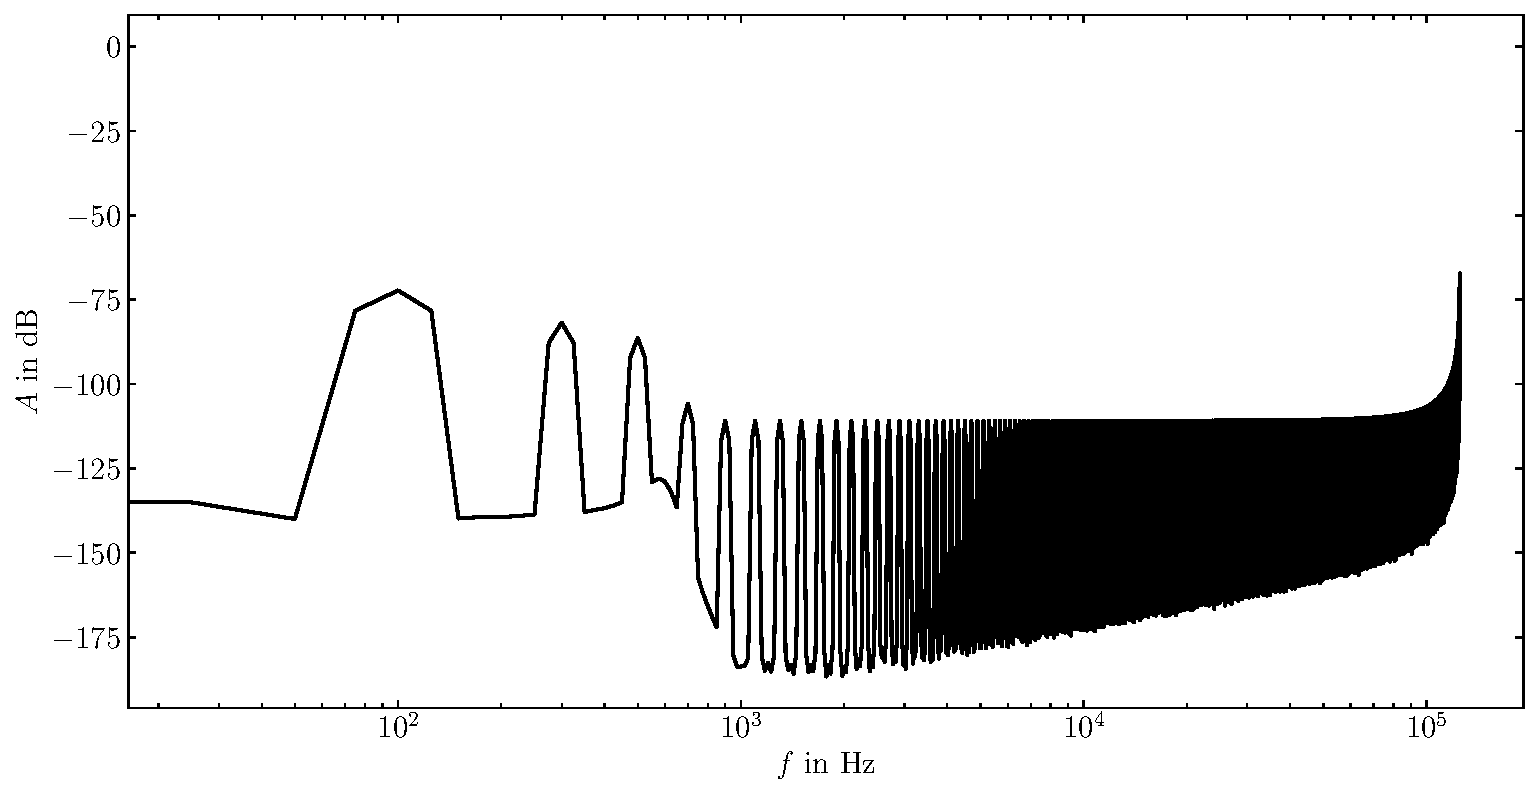
\includegraphics[width=\textwidth]{Paul/43bInChHi1F.pdf}
        \caption{Fourierspektrum}
    \end{subfigure}
    \caption{Inverser Chebyshevfilter als Hochpass}
    \label{fig:43bInChHi1}
\end{figure}

\newpage
In Abbildung \ref{fig:43bInChLo1} fällt die konstante Nulllinie beim gefilterten Signal auf, auch ist das abknicken (bei ca. 1 kHz), im Vergleich zum Butterworthtiefpass ausgeprägter.\\

\begin{figure}[h]
    \centering
    \begin{subfigure}{0.9\textwidth}
        \centering
        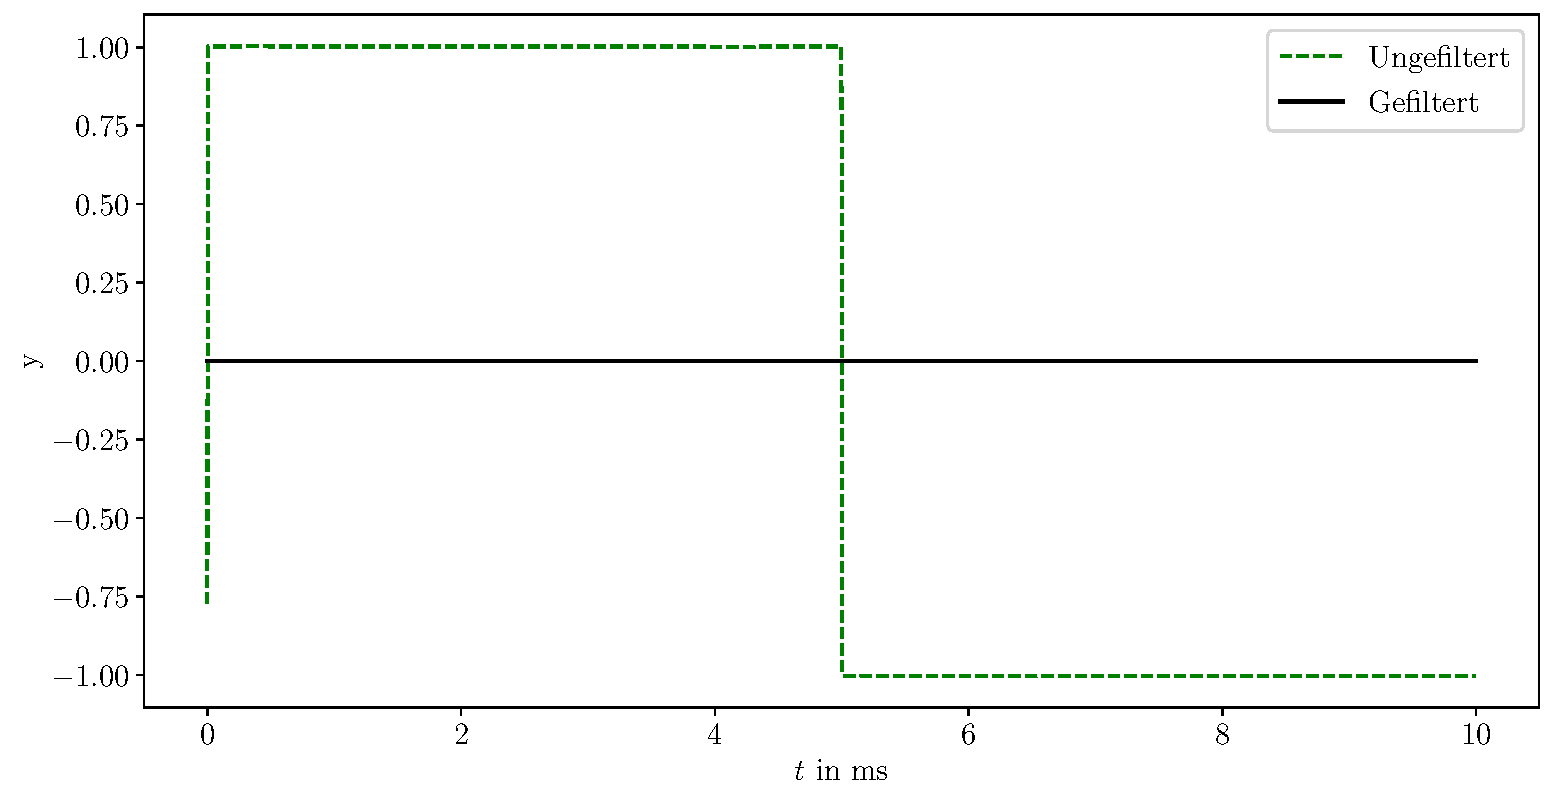
\includegraphics[width=\textwidth]{Paul/43bInChLo1S.pdf}
        \caption{Signal}
    \end{subfigure}
    \\
    \begin{subfigure}{0.9\textwidth}
        \centering
        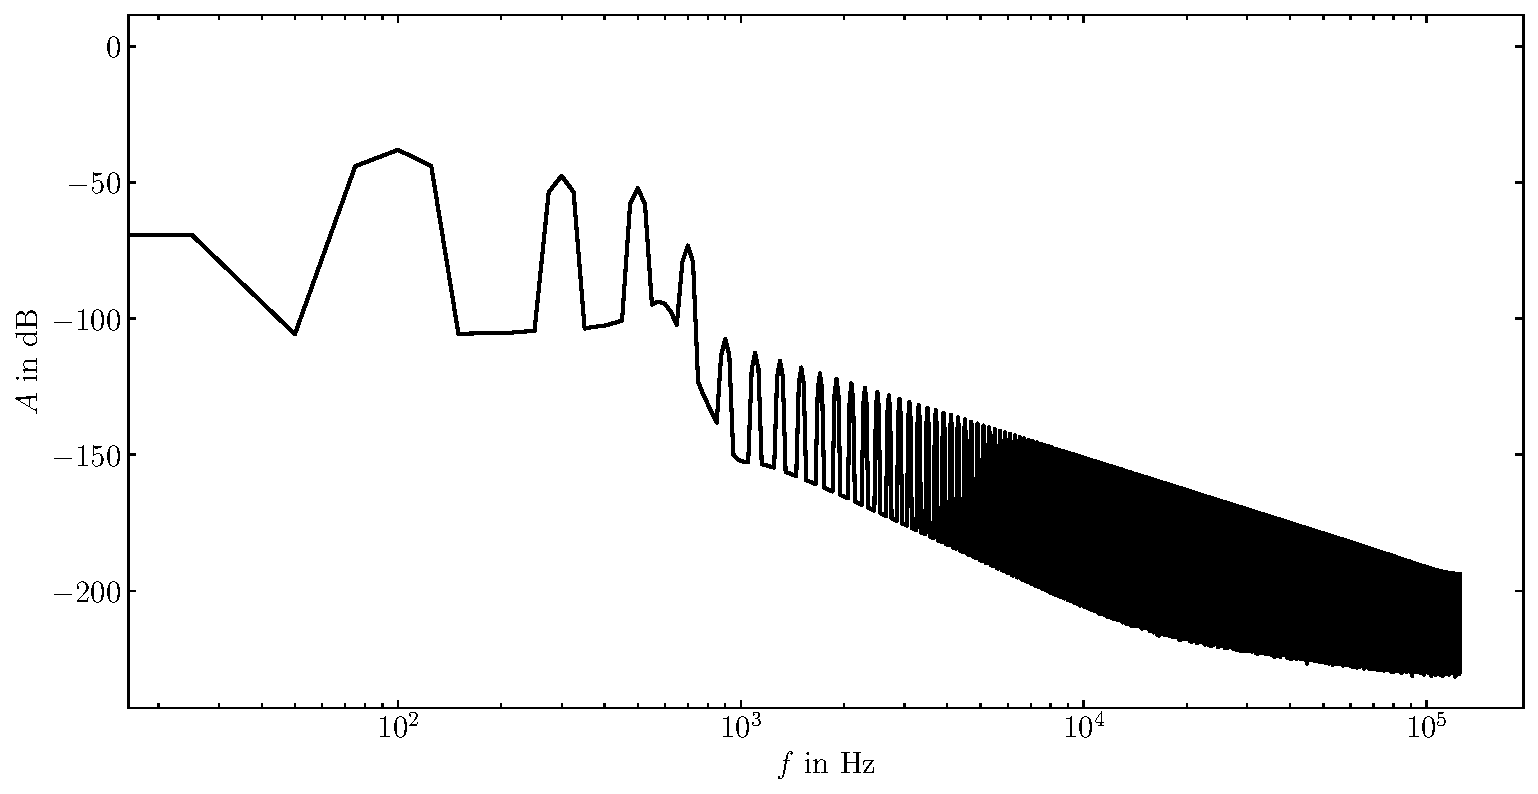
\includegraphics[width=\textwidth]{Paul/43bInChLo1F.pdf}
        \caption{Fourierspektrum}
    \end{subfigure}
    \caption{Inverser Chebyshevfilter als Tiefpass}
    \label{fig:43bInChLo1}
\end{figure}

Da die anderen Filter ähnliche Eigenschaften wie der Butterworthfilter aufweisen wurde auf die Abbildung deren Signale und Fourierspektren bewusst verzichtet.\\

\newpage
\subsection{Bandpass 4. Ordnung}

In diesem Abschnitt soll die geeignete Einstellung eines Butterworthbandpasses (4. Ordnung) gefunden werden, die Rauschen, beim gleichzeitigen Erhalt der zeitlichen Form der Signalfunktion, abmildert.
\begin{figure}[h]
    \centering
    \begin{subfigure}{0.9\textwidth}
        \centering
        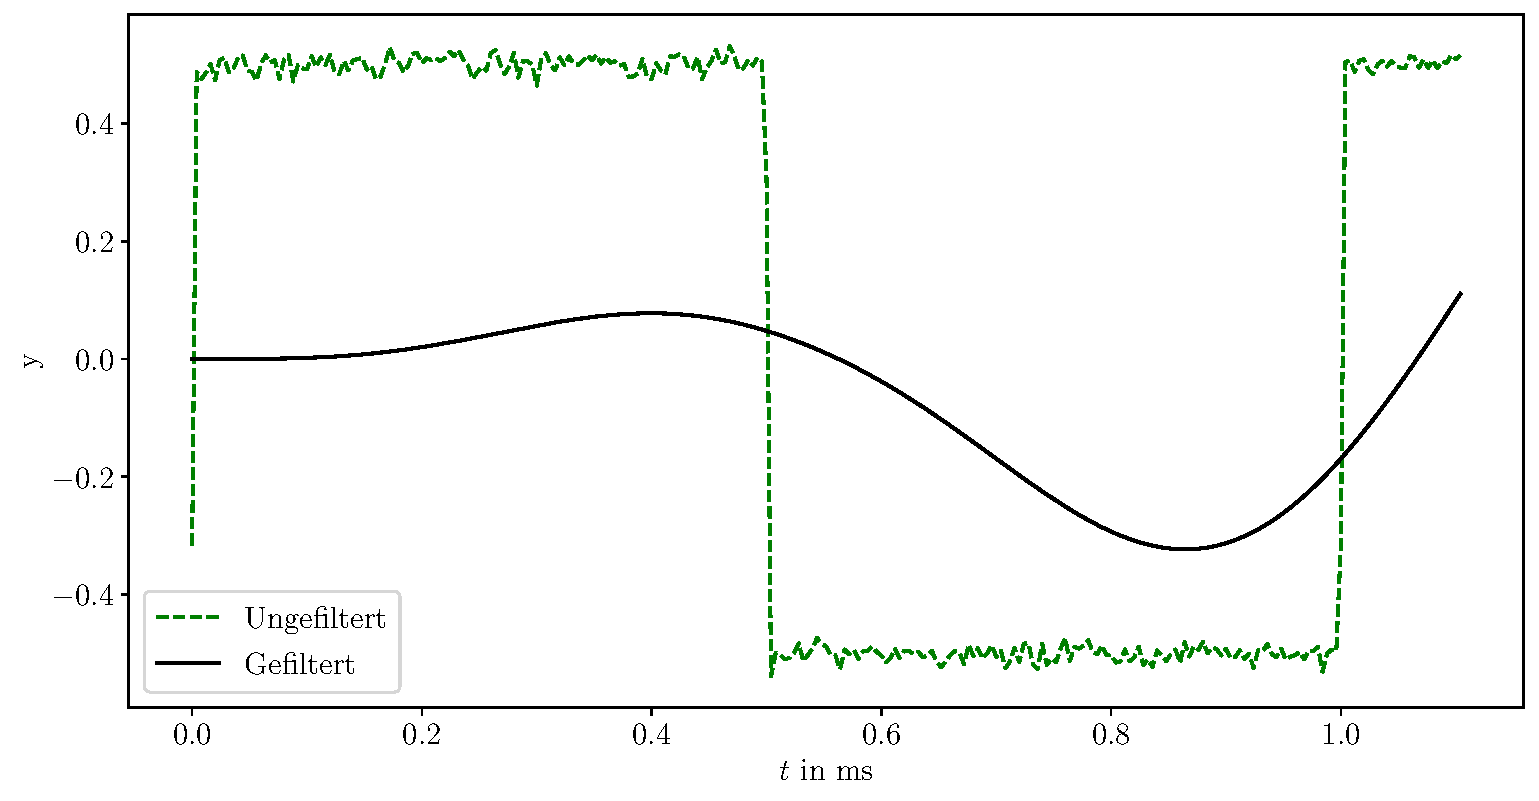
\includegraphics[width=\textwidth]{Paul/43cLf500Hf1500S.pdf}
        \caption{Bandpass mit Durchlassbereich von 500 bis 1500Hz}
    \end{subfigure}
    \\
    \begin{subfigure}{0.9\textwidth}
        \centering
        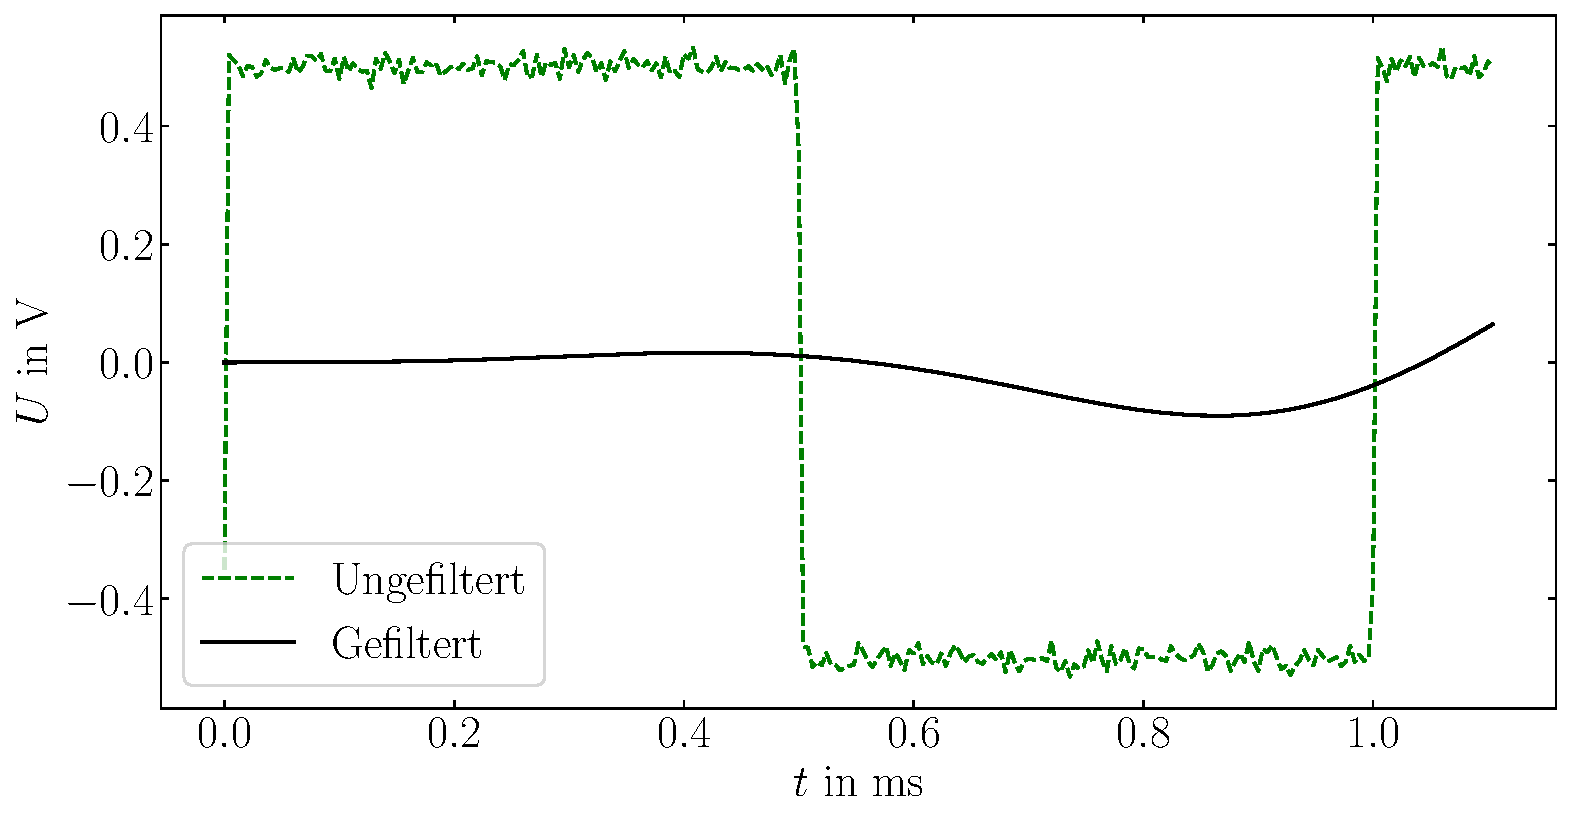
\includegraphics[width=\textwidth]{Paul/43cLf700Hf1300S.pdf}
        \caption{Bandpass mit Durchlassbereich von 700 bis 1300Hz}
    \end{subfigure}
    \caption{Signalfunktion verschiedener Bandpässe}
    \label{fig:43cverBa}
\end{figure}

Die in Abbildung \ref{fig:43cverBa} gezeigten Signalfunktionen weichen stark von einer Rechteckfunktion ab und sind daher ungeeignet.\\
Durch weiteres Ausprobieren wurden bessere Einstellungen gefunden, welche die in Abbildung \ref{fig:43cBeBa} dargestellte Signalfunktion ergeben. Hier ist noch deutlich ein Rechtecksignal zu erkennen.\\

\begin{figure}[h]
    \centering
    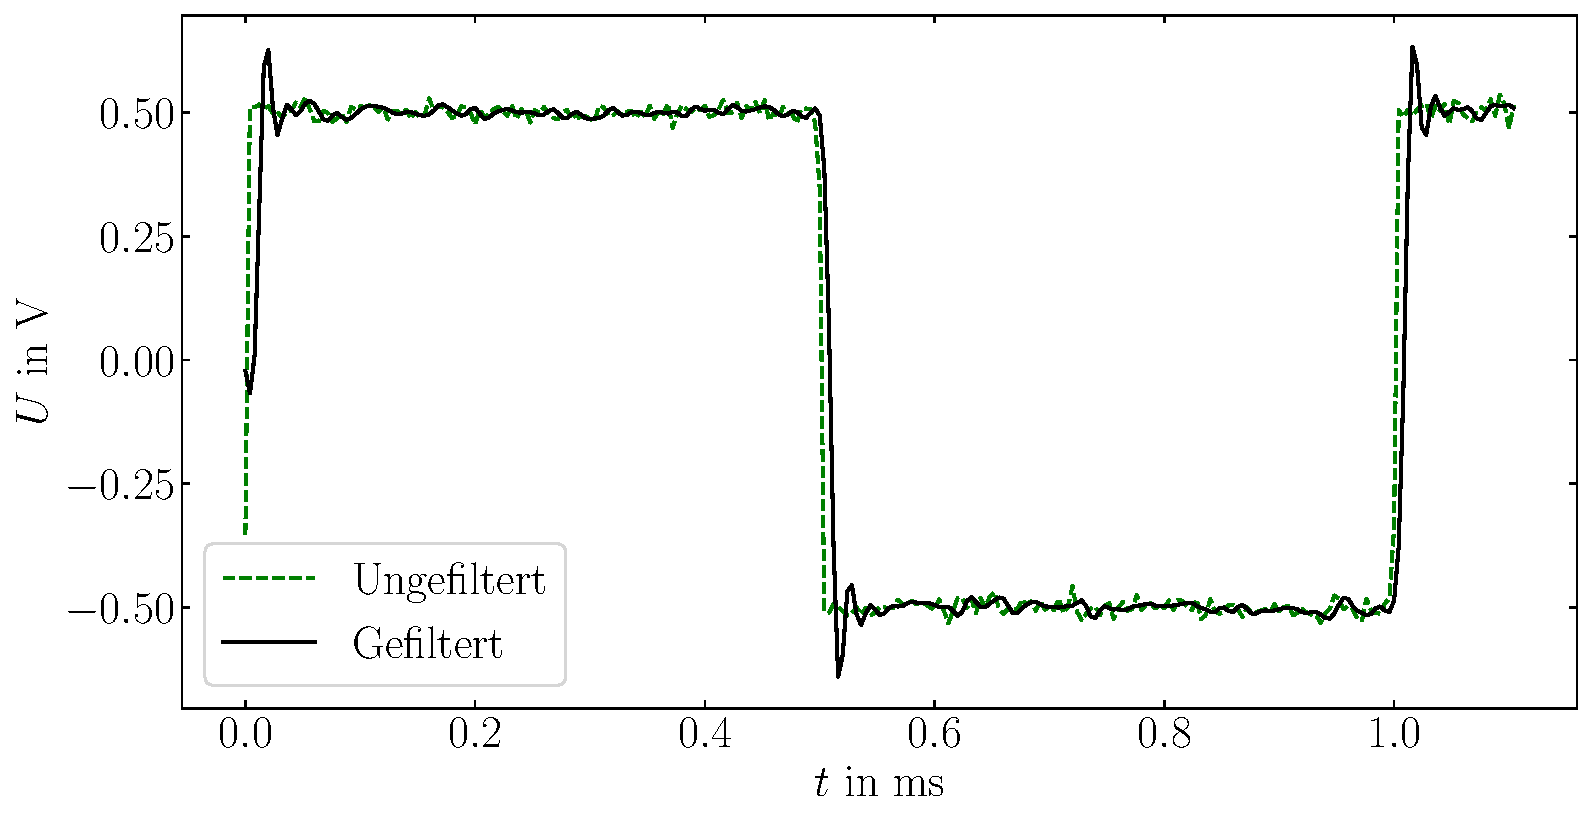
\includegraphics[width=\textwidth]{Paul/43cLf10mHz55kHzS.pdf}
    \caption{Bandpass mit Durchlassbereich von 10mHz bis 55kHz}
    \label{fig:43cBeBa}
\end{figure}

Eine gute Rauschunterdrückung verursacht also eine große Signalverzerrung. Der Grund hierfür ist folgender: Die Fouriertransformierte des Rechtecksignals ist eine Superposition von Sinusschwingungen über den ganzen Frequenzraum, wenn nun ein Teil dieser Frequenzen herausgefiltert werden und eine Rücktransformation erfolgt kommt es, aufgrund der fehlenden Frequenzen zu einer Signalverzerrung. Das heist um so enger der Bandpass eingestellt wird um so verzehrter wird das Rechtecksignal, was gut zu unseren Beobachtungen passt. Es ist also darauf zu achten, dass dieses Verhältnis, abhängig vom Fokus der Messung, klug gewählt wird.

\newpage
\subsection{Einfluss der Ordnung}
\label{chap:Einfl-d-Ord}
Im folgenden soll betrachtet werden welchen Einfluss die Ordnung eines Filters hat.
Um diesen Umstand genauer betrachten zu können werden Fourierspektren von Filtern verschiedener Ordnung miteinander verglichen.
\begin{figure}[h]
    \centering
    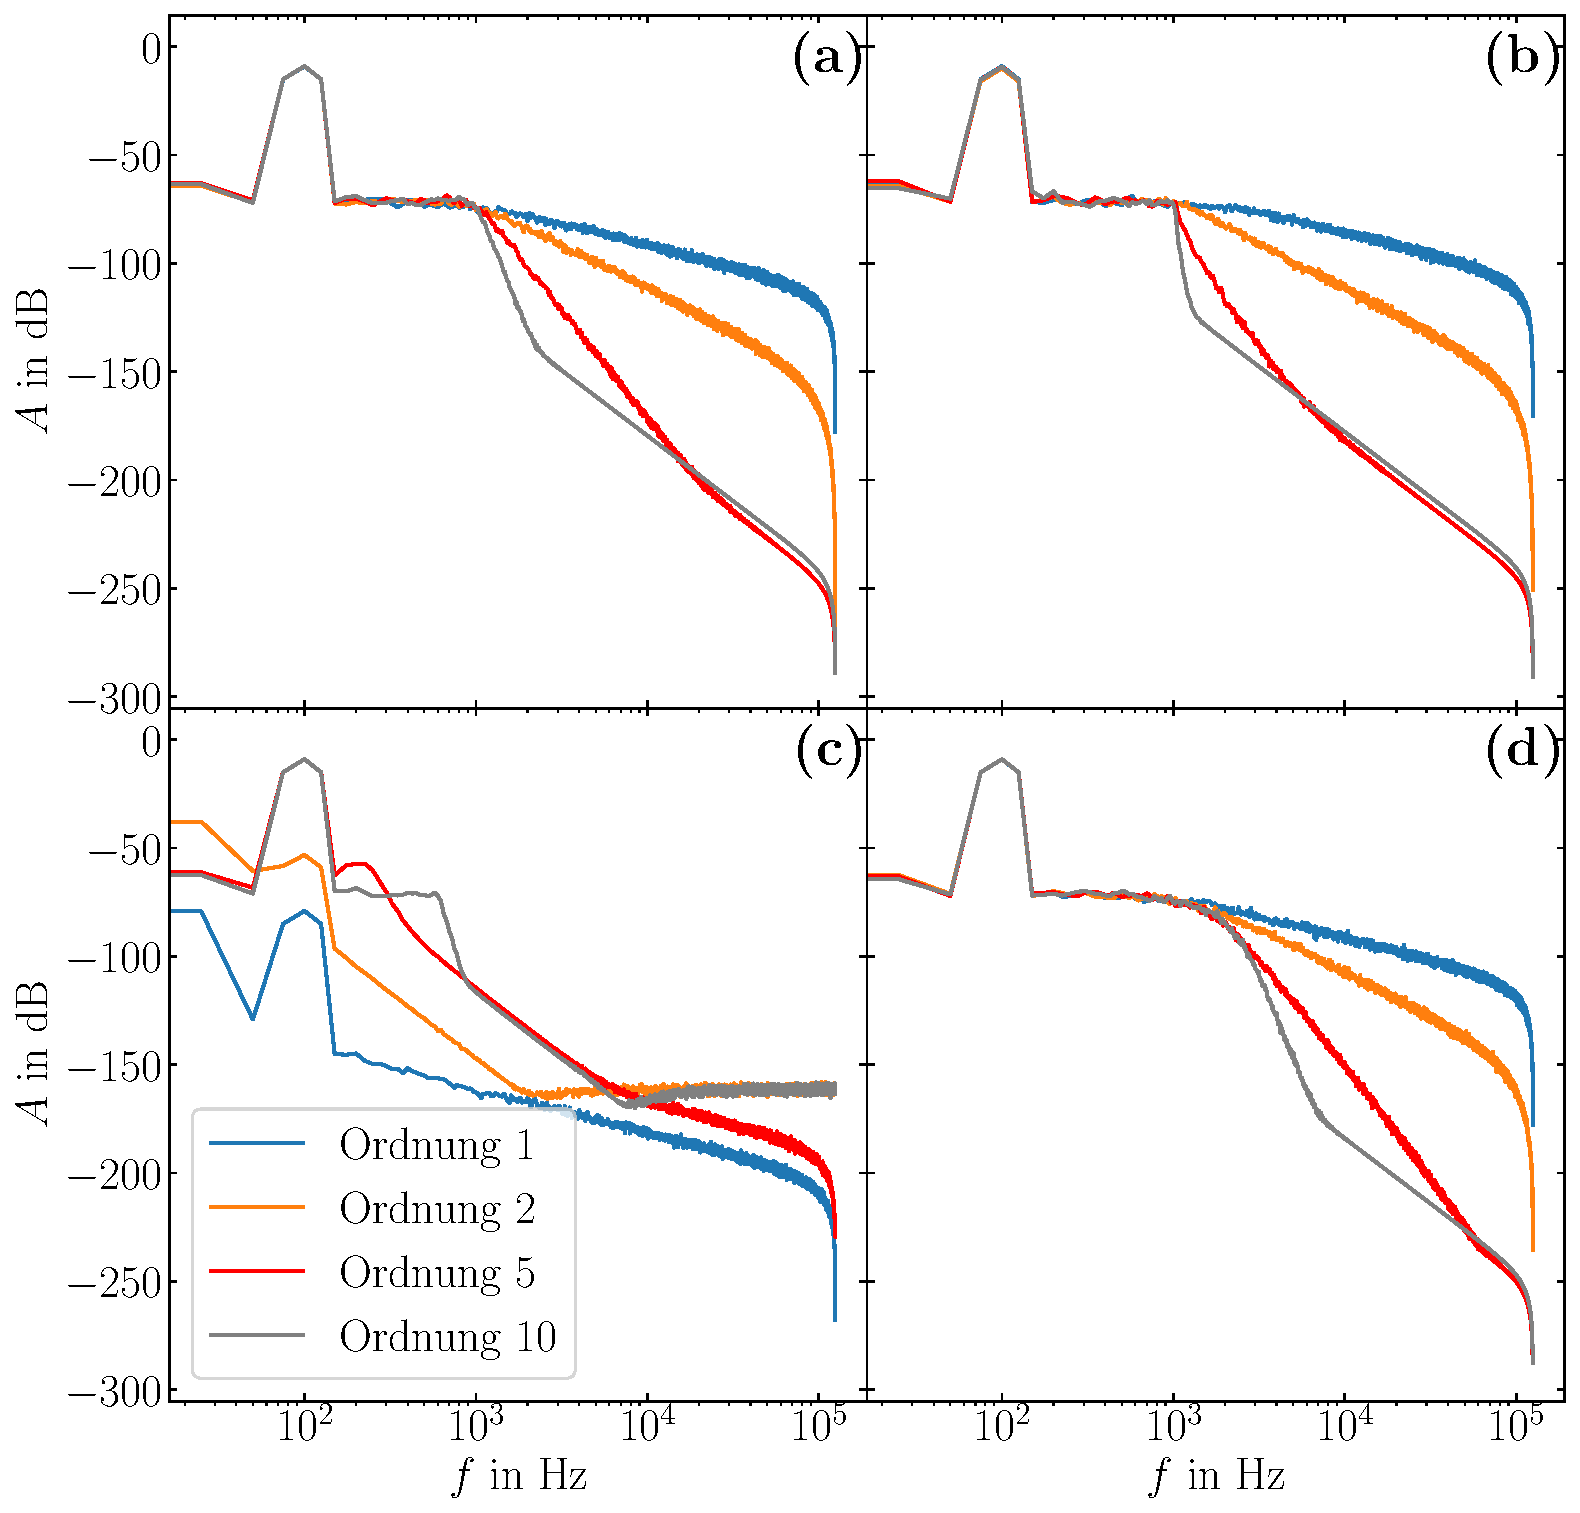
\includegraphics[scale = 0.5]{Paul/43dAllFilAll.pdf}
    \caption{(a) Butterworth, (b) Chebyshev, (c) Inverse Chebyshev und (d) Besselfilter bei verschiedenen Ordnungen}
    \label{fig:43dOrd}
\end{figure}

Aus Abbildung \ref{fig:43dOrd} ist zu erkennen, dass mit höherer Ordnung die Kurve, nach dem Knick, steiler Abfällt.
Für große Ordnungen fällt jedoch ein weiterer Knick bei höheren Frequenzen auf, welcher die Kurve danach abflacht. Außerdem sind alle Filter im Durchlassbereich, unabhängig von der Ordnung, deckungsgleich, bis auf den Inversen Chebyshev. Beim Inversen Chebyshev ist auch noch zu beobachten, dass für gerade Ordnungen, die Kurve im letzten Teil des Frequenzspektrums waagrecht verläuft.

\newpage
\subsection{Vergleich: Analoge und digitale Filterung}
Um die analoge mit der digitalen Filterung zu Vergleichen wird zuerst eine Messung mit dem gewohntem Messaufbau für den digitalen Filter aufgenommen. Danach wird der digitale Filter über die Messsoftware deaktiviert und zwischen den Generator und Detektor wird ein analoger Filter (Modell: Ithaco 4302) geschaltet, der analog zum digitalen Filter eingestellt wurde.

\begin{figure}[h]
    \centering
    \begin{subfigure}{0.9\textwidth}
        \centering
        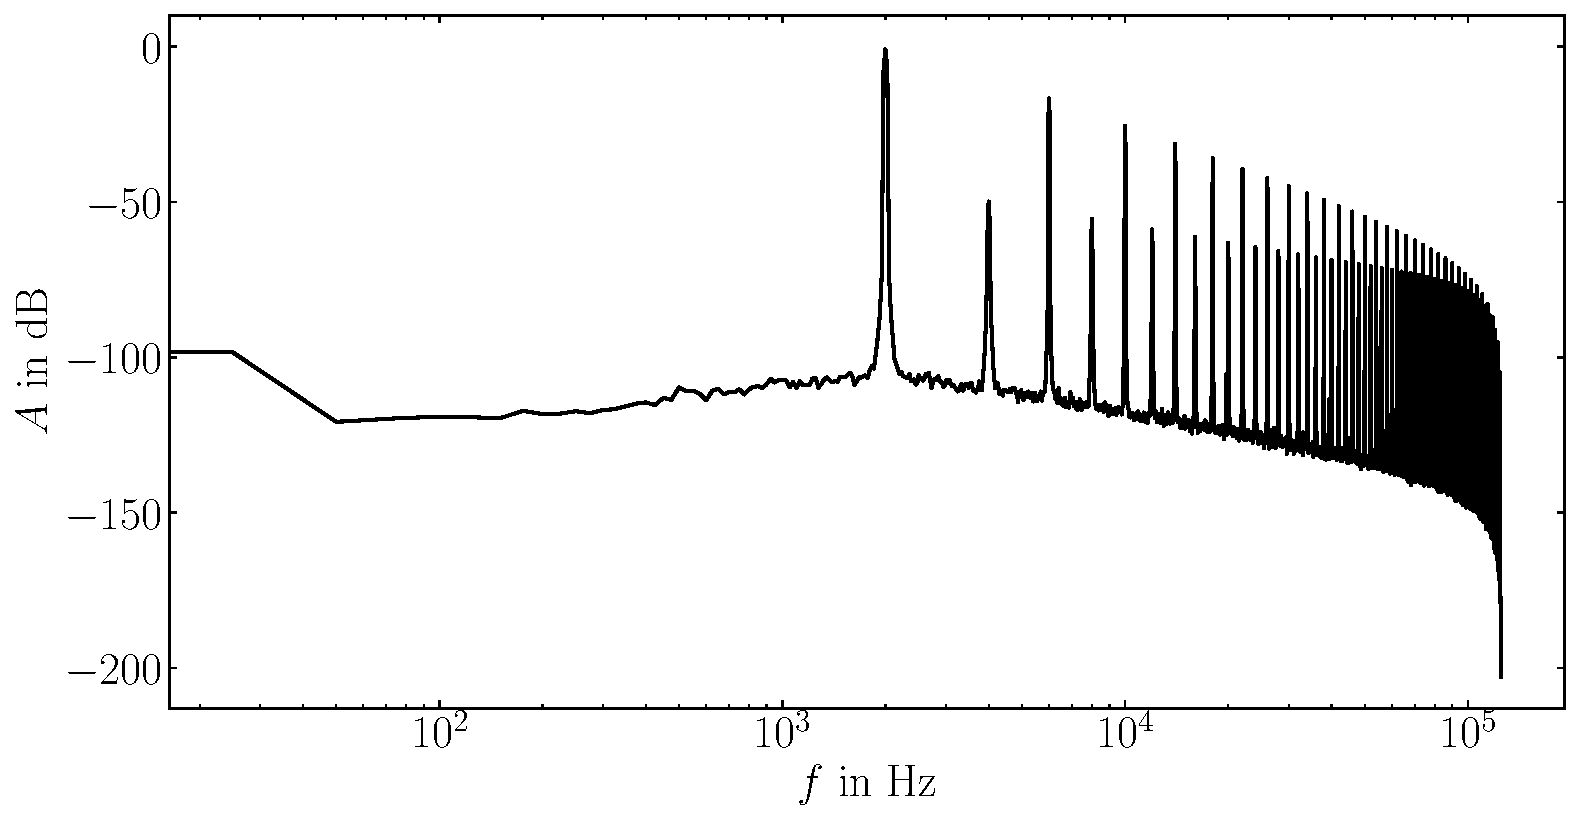
\includegraphics[width=\textwidth]{Paul/43eDF.pdf}
        \caption{digitale Filterung}
    \end{subfigure}
    \\
    \begin{subfigure}{0.9\textwidth}
        \centering
        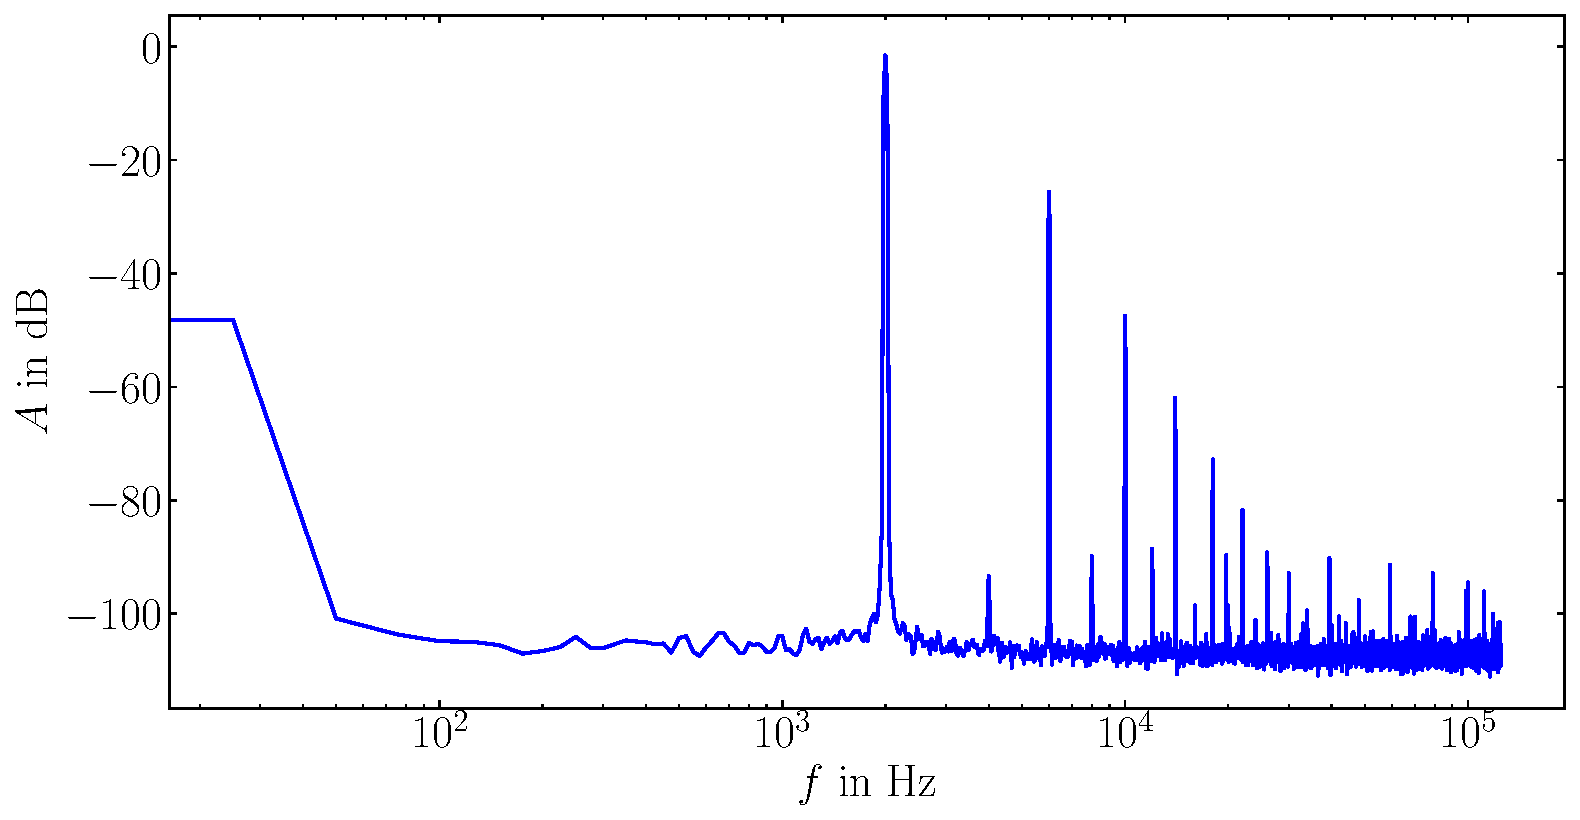
\includegraphics[width=\textwidth]{Paul/43eAF.pdf}
        \caption{analoge Filterung}
    \end{subfigure}
    \caption{Vergleich von analoger und digitaler Filterung}
    \label{fig:43e}
\end{figure}
\newpage
In Abbildung \ref{fig:43e} sind die Fourierspektren nach analoger und digitaler Filterung aufgetragen. Vergleicht man beides, so fällt auf, dass bei der digitalen Filterung auch der Hintergrund die Charakteristik des Bandpasses zeigt, wohingegen bei der analogen Filterung scheinbar nur die Nebenmaxima betroffen sind.\\
Eine mögliche Erklärung wäre, dass der Hintergrund nach dem analogen Filter einkoppelt oder das diese Eigenschaft eine Eigenschaft des analogen Filters ist, bzw. die Auflösung der Filter ab -100dB abnimmt. (Aus Gründen der Übersichtlichkeit wurde darauf verzichtet, die Kurven in einen einzigen Plot aufzuzeichnen.)


\subsection{Vergleich Filterung und Mittelung}
Wenn man Filterung und Mittelung gegenüberstellt, so ist der größte Unterschied wohl das beim Filtern aktiv bestimmte Frequenzen unterdrückt werden, je nach Einstellung bzw. Dimensionierung des Filters. Dies kann dabei helfen, dass das Messsignal von Störungen wie dem 50\,Hz Brummen bereinigt werden kann.\\
Mitteln hingegen ist besonders geeignet um die Messung von bspw. weißes Rauschen zu bereinigen da dies, gemittelt über die Zeit, Null ergibt.